\PassOptionsToPackage{unicode=true}{hyperref} % options for packages loaded elsewhere
\PassOptionsToPackage{hyphens}{url}
%
\documentclass[]{article}
\usepackage{lmodern}
\usepackage{amssymb,amsmath}
\usepackage{ifxetex,ifluatex}
\usepackage{fixltx2e} % provides \textsubscript
\ifnum 0\ifxetex 1\fi\ifluatex 1\fi=0 % if pdftex
  \usepackage[T1]{fontenc}
  \usepackage[utf8]{inputenc}
  \usepackage{textcomp} % provides euro and other symbols
\else % if luatex or xelatex
  \usepackage{unicode-math}
  \defaultfontfeatures{Ligatures=TeX,Scale=MatchLowercase}
\fi
% use upquote if available, for straight quotes in verbatim environments
\IfFileExists{upquote.sty}{\usepackage{upquote}}{}
% use microtype if available
\IfFileExists{microtype.sty}{%
\usepackage[]{microtype}
\UseMicrotypeSet[protrusion]{basicmath} % disable protrusion for tt fonts
}{}
\IfFileExists{parskip.sty}{%
\usepackage{parskip}
}{% else
\setlength{\parindent}{0pt}
\setlength{\parskip}{6pt plus 2pt minus 1pt}
}
\usepackage{hyperref}
\hypersetup{
            pdfborder={0 0 0},
            breaklinks=true}
\urlstyle{same}  % don't use monospace font for urls
\setlength{\emergencystretch}{3em}  % prevent overfull lines
\providecommand{\tightlist}{%
  \setlength{\itemsep}{0pt}\setlength{\parskip}{0pt}}
\setcounter{secnumdepth}{0}
% Redefines (sub)paragraphs to behave more like sections
\ifx\paragraph\undefined\else
\let\oldparagraph\paragraph
\renewcommand{\paragraph}[1]{\oldparagraph{#1}\mbox{}}
\fi
\ifx\subparagraph\undefined\else
\let\oldsubparagraph\subparagraph
\renewcommand{\subparagraph}[1]{\oldsubparagraph{#1}\mbox{}}
\fi

\usepackage{graphicx}
\usepackage[left=2cm,right=2cm]{geometry}

% set default figure placement to htbp
\makeatletter
\def\fps@figure{htbp}
\makeatother

\newcommand{\mbf}{\mathbf}

\begin{document}

\title{Neuro 120 HW1}
\author{Sam Lurye, Gerardo Parra}
\date{October 4, 2018}
\maketitle

\section*{Problem 1}

\textbf{(a)} See code.
\\\\
\textbf{(b)} When $\Delta t=0.09$, the approximation diverges: the step size is too large, and so our Euler integrator does not effectively approximate the solution to the differential equations, instead returning massive numbers. When $\Delta t=0.07$, the approximation converges; however, the plot of membrane potential is more jagged than when $\Delta t=0.01$.

\section*{Problem 2}

Shortly after the input current is applied, the sodium channel gating variable $m$ begins to increase, so sodium ions begin flowing into the neuron, raising the membrane potential. This in turn causes $m$ to increase even more, beginning a chain reaction, so that the membrane potential jumps rapidly to a peak. Shortly after $m$ begins increasing, $h$ begins to decrease and $n$ begins to increase. The decrease in $h$ corresponds to the inactivation of sodium channels, meaning less sodium flows into the neuron. Meanwhile, the increase in $n$ corresponds to potassium ions flowing out of the neuron. $n$ and $h$ together cause the membrane potential to begin to fall, and as this happens, $m$ begins to decrease, causing the membrane potential to drop even further. Eventually, so much potassium has flowed out of the neuron that the membrane potential is more negative than its resting state. When this happens, $n$ begins to decrease and $h$ begins to increase, so that potassium stops leaving the cell and sodium can begin flowing in again. As a result, the membrane potential is slowly restored to its initial resting state.

\section*{Problem 3}

\textbf{(a) and (b)} The following is a plot of firing rate in Hz versus current in $\mu A$. The minimum sustained firing rate for the HH model is about 53.48 Hz.

\begin{figure}
    \centering
    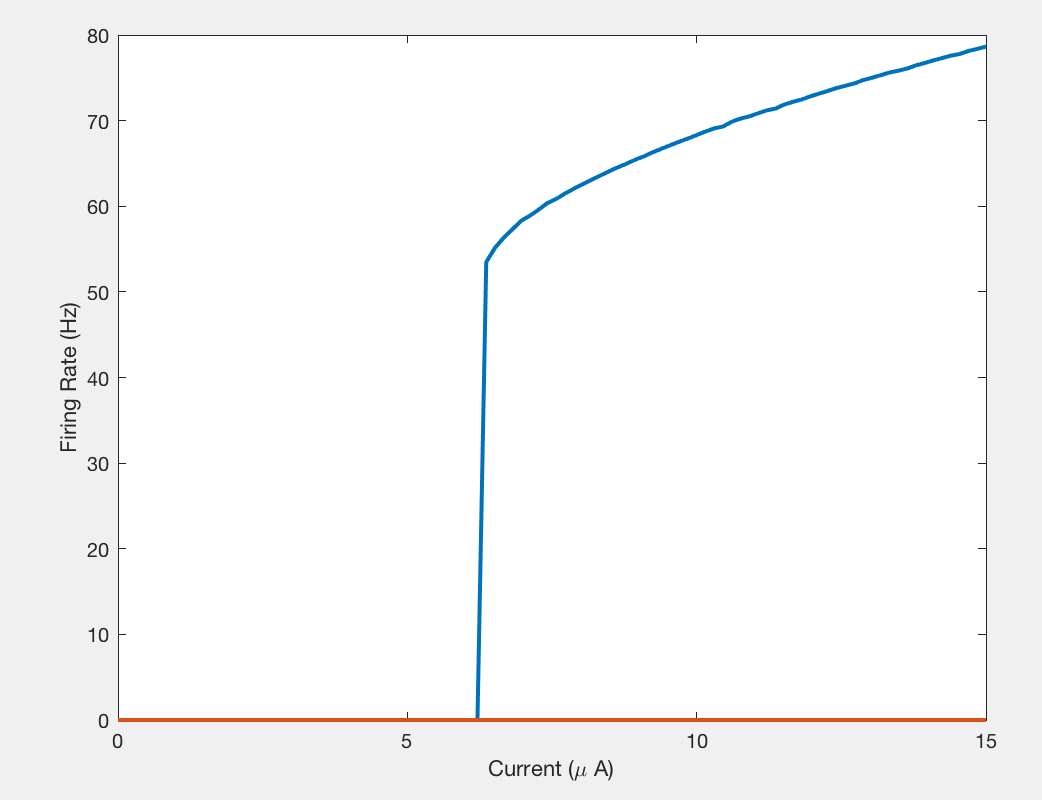
\includegraphics[scale=0.5]{const_current_firing_rate.png}
    \label{fig:const_current}
\end{figure}

\section*{Problem 4}

\textbf{(a)} Two spikes are fired in response to two pulses separated by 12ms.
\\\\

\textbf{(b)} A single spike is fired in response to two pulses separated by 3ms.
\\\\

\textbf{(c)} For the pulses separated by 3ms, the second pulse occurs at 13 ms just as the sodium channel inactivation variable $h$ is approaching its lowest values, indicating that sodium channels are at the greatest probability of being inactivated. The neuron is thus in the refractory period, which prevents the cell from firing another spike. Since the pulse only lasts 2 ms, the current returns to normal by the time the cell can support another action potential.
\begin{figure}
    \centering
    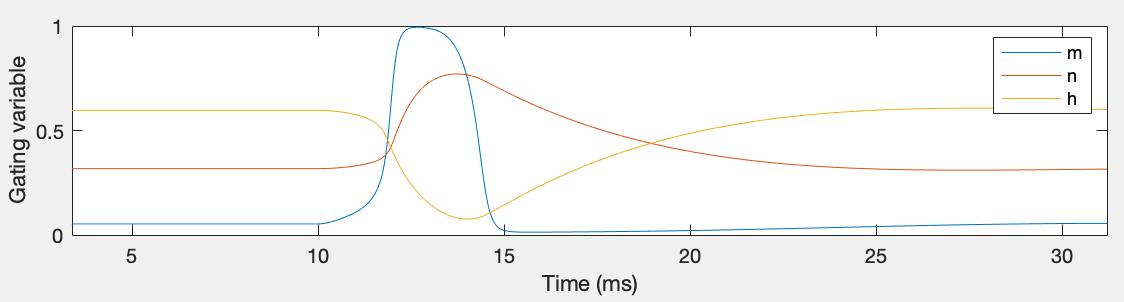
\includegraphics[scale=0.5]{gating3ms.png}
    \label{fig:gating3ms}
\end{figure}

For the pulses with 12ms separation, the second pulse occurs at 22 ms when all gating variables $m,n,h$ have returned to their default values. This indicates that the neuron is at rest and capable of firing, so the second pulse causes a spike.
\begin{figure}
    \centering
    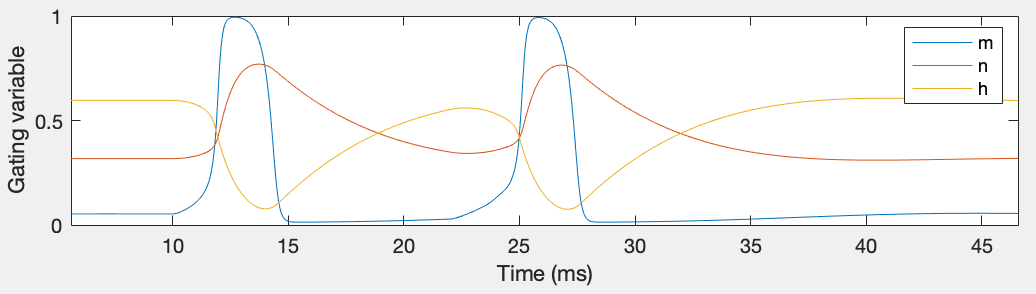
\includegraphics[scale=0.5]{gating12ms.png}
    \label{fig:gating12ms}
\end{figure}


\section*{Problem 5}
\textbf{(a)} The firing rate after the rise to 8 $\mu A$ is 62.4257 Hz.
\\\\
\textbf{(b)} The firing rate after the drop to 8 $\mu A$ is 0 Hz.
\\\\
\textbf{(c)} The firing rate is 0 Hz for higher currents--the firing rate in 3a is only 0 Hz for currents less than 6 $\mu A$, while the rate is 0 Hz here for currents up to 8 $\mu A$. This is an example of how history affects spikes, by changing the state of the gating variables at the time of of pulse.

\begin{figure}
    \centering
    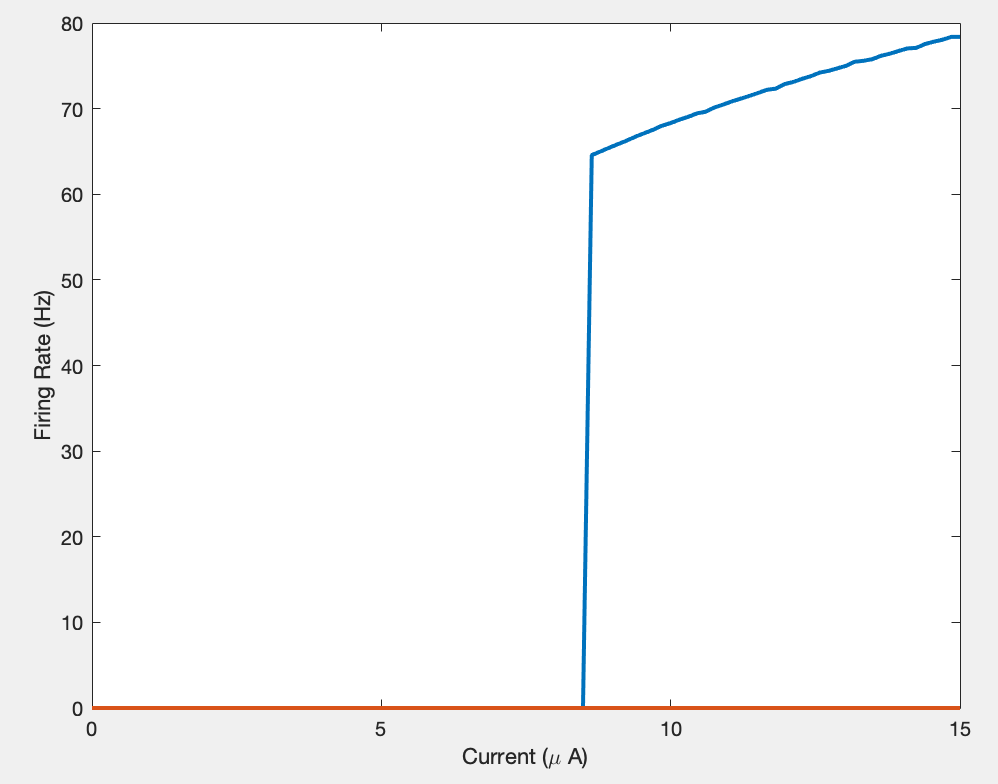
\includegraphics[scale=0.5]{history_firing_rate.png}
    \label{fig:history_rate}
\end{figure}

\textbf{(d)} The initial spike is stronger because the gating variables begin at $m$ = 0.0529, $n$ = 0.3177, $h$=0.5961, but since the current remains at 10 $\mu A$, the neuron continues fire immediately after exiting the refractory period and before the gating variables can fully return to their default state. Specifically, at each subsequent spike, the sodium channel inactivation variable is lower than its default state and the potassium channel activation variable is slightly higher, so repolarization occurs earlier.

\begin{figure}
    \centering
    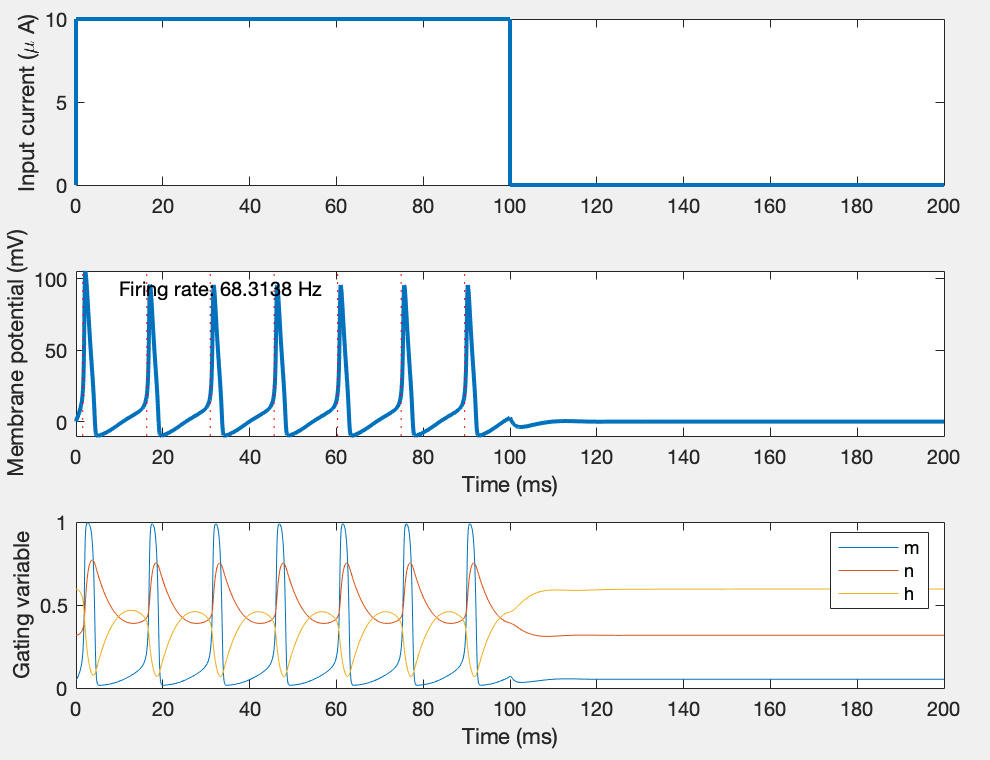
\includegraphics[scale=0.75]{history_dependence.png}
    \label{fig:history}
\end{figure}

The slight activity at 100 ms isn't a spike because the current is turned off before threshold voltage for a spike is reached.

\section*{Problem 6}
\textbf{(a)} The firing rate for $\omega = 2\pi\frac{50}{1000}$ is 50.0156 Hz. As seen in the figure below, the firing rate has a complex relationship with $\omega$:
\begin{figure}
    \centering
    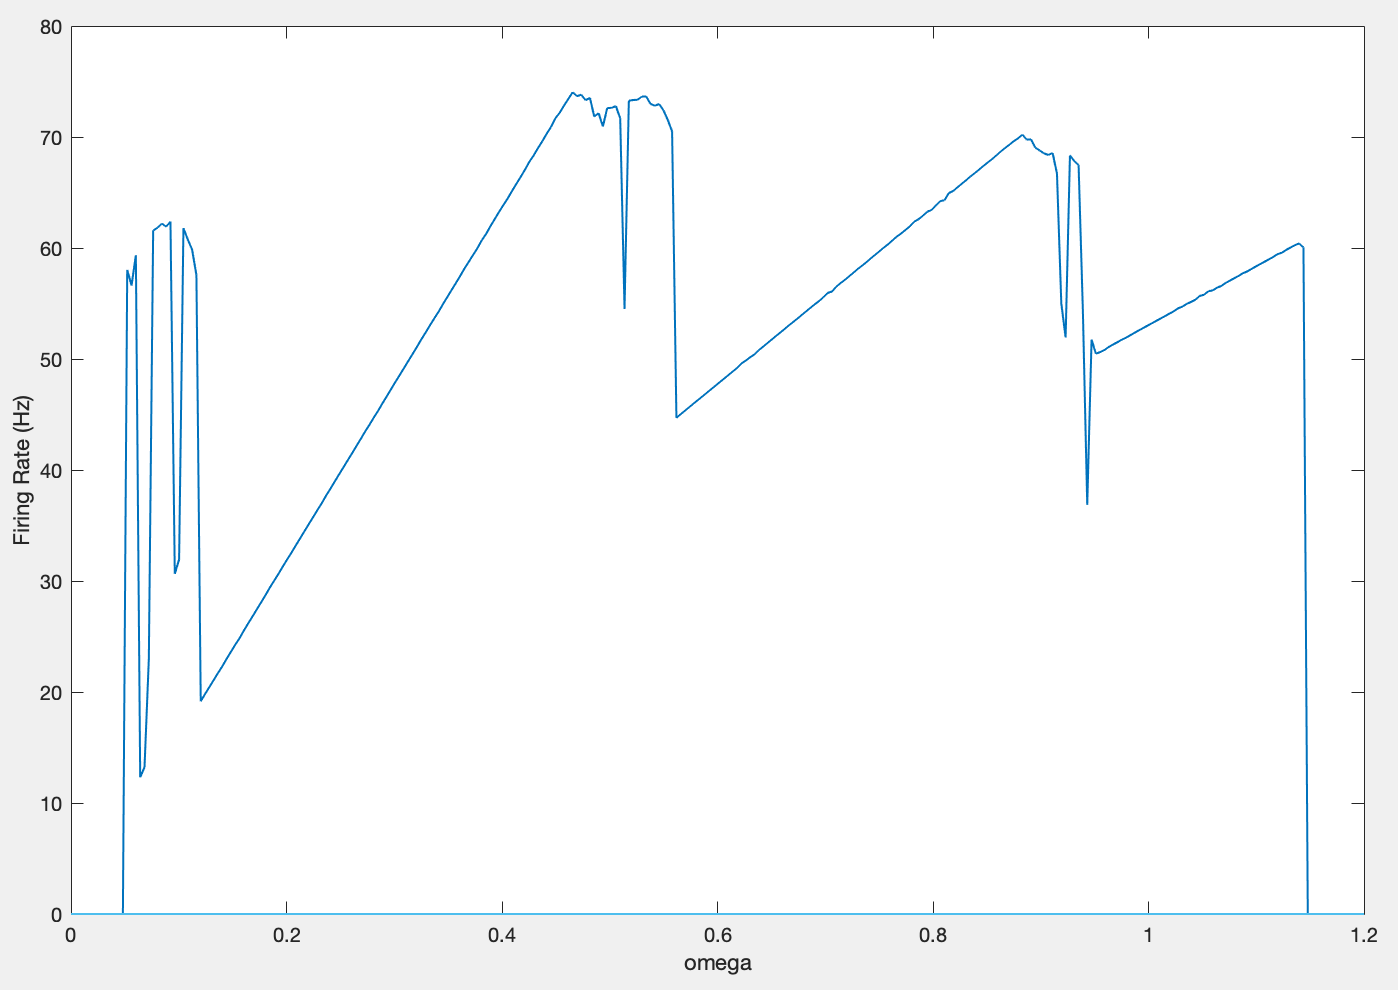
\includegraphics[scale=0.4]{omega.png}
    \label{fig:omega}
\end{figure}

\textbf{(b)}
\begin{figure}
    \centering
    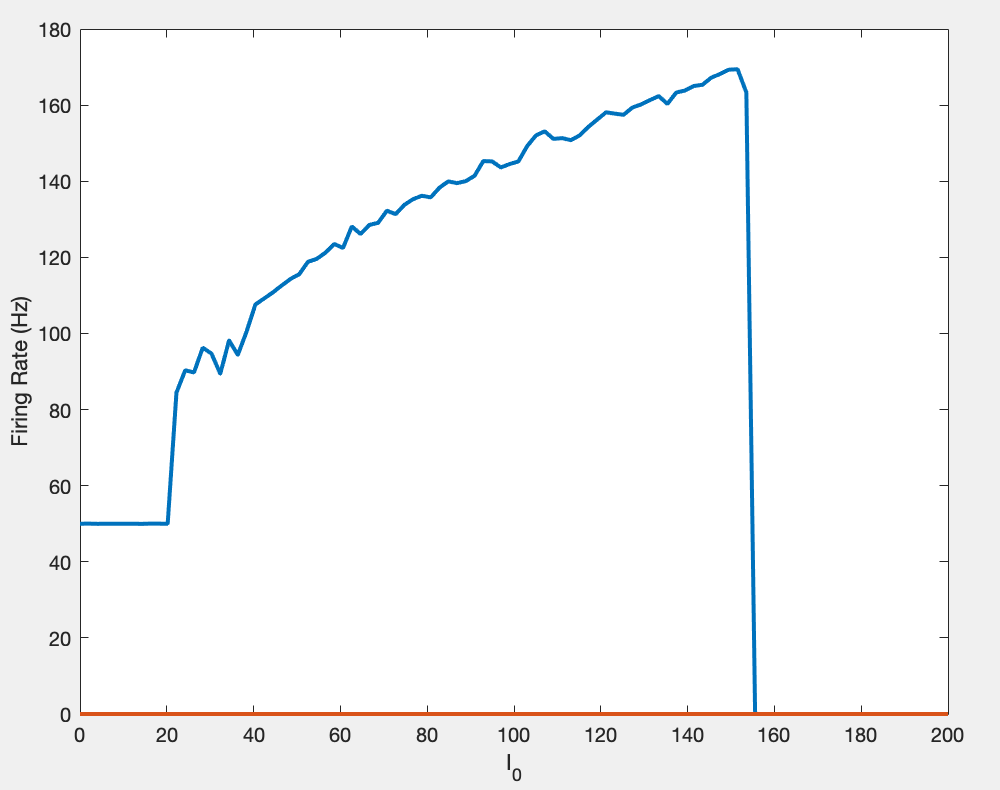
\includegraphics[scale=0.5]{i0_firing_curve.png}
    \label{fig:i0_curve}
\end{figure}

\textbf{(c)} $I_0$ has no effect on the firing rate in this range.
\begin{figure}
    \centering
    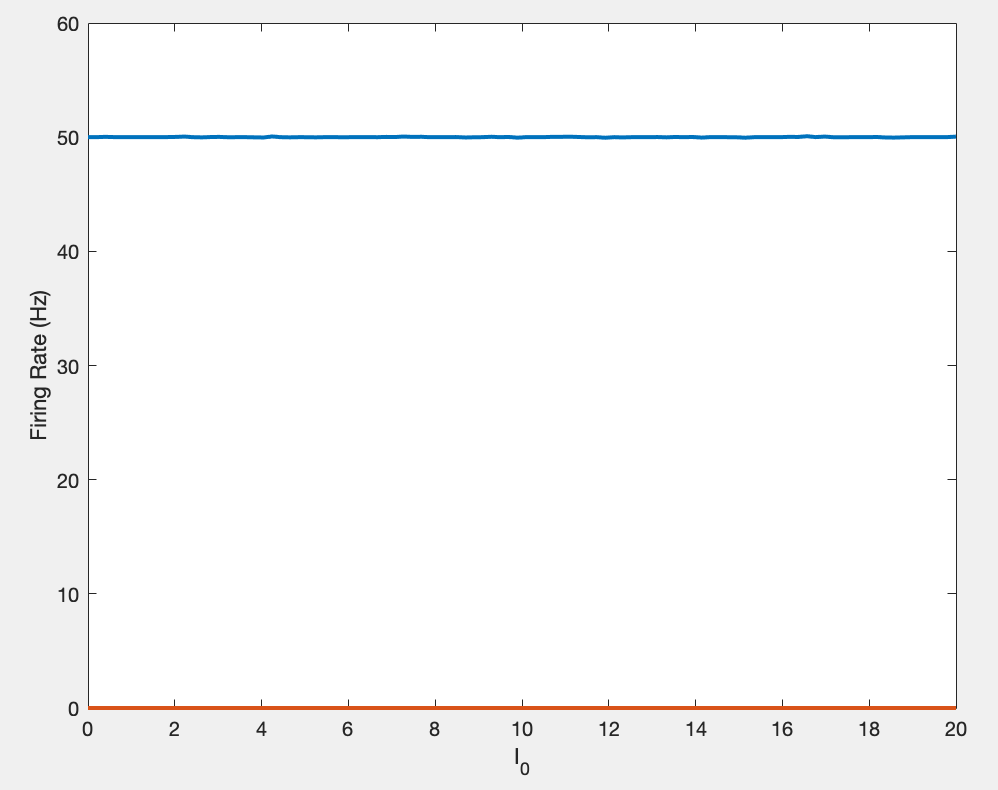
\includegraphics[scale=0.5]{i0_range.png}
    \label{fig:i0_range}
\end{figure}

\end{document}
